%!TEX root = ../thesis.tex
%*******************************************************************************
%****************************** Second Chapter *********************************
%*******************************************************************************

\chapter{Designing User-Centric ML Systems}
\label{chapter2}

\graphicspath{{Chapter2/figs/}}

This chapter focuses on describing some advances in the context of Interactive ML and Interpretable ML. In first instance, both sub-fields are tackled independently but, in Section \ref{section2.3}, a discussion is stated in terms of how they can be combined for designing better and more user-centric ML systems.

\section{Interactive ML}
\label{section2.1}

The Human-Computer Interaction (HCI) field cares about human perception, cognition, intelligence, decision-making and interactive techniques of visualization. By the other hand, in Knowledge Discovery in Databases (KDD) automatic computational methods for finding previously unknown relationships in data are developed \cite{Holzinger2013}. By merging these fields, many research opportunities emerge including the paradigm where algorithms can interact with humans and optimize their learning behavior through these interactions \cite{Holzinger2016}. 

As described in \cite{Fails2003}, classic ML generally has some assumptions which can be addressed through the use of Interactive ML, such as:

\begin{itemize}
\item The introduction of many attributes in the model can become noise and therefore affect its performance. An Interactive ML system should provide to user the ability to perform attribute selection through a friendly interface.
\item When there is not enough training data, user also should be able to perform labeling under consideration or by a systematic way.
\item The system must quickly adapt after any user interaction affecting the data or model behavior. A delayed adaptation implies losing the user's attention.
\end{itemize}

More formally, Interactive ML is a co-adaptive process, driven by the user, but inherently dynamic in nature as the model and user evolve together during training \cite{Dudley2018}. These kind of systems should include interaction elements: \textbf{sample review}, \textbf{feedback assignment}, \textbf{model inspection} and \textbf{task overview}. By the other hand, an interface for Interactive ML should meet the following requirements: train very quickly, accommodate hundreds to thousands of features, perform feature selection and support tens to hundreds of thousands of training examples \cite{Fails2003}. A synthesis of a Interactive ML system is shown in Figure \ref{fig:InteractiveML} describing the direction of the interaction for each element. 

\begin{figure}[ht]
 \centering
 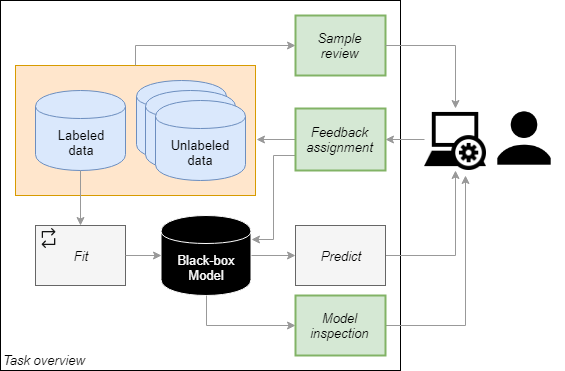
\includegraphics[width=0.7\textwidth]{InteractiveML.png}
 \caption{Block diagram representing an Interactive ML system.}
 \label{fig:InteractiveML}
\end{figure}

Known strategies for implementing the first two elements are briefly described in Subsections \ref{subsection2.1.1} and \ref{subsection2.1.2}. Although the \textbf{model inspection} element apparently does not have the same level of development, some relevant works are presented in Subsection \ref{subsection2.1.3}. For \textbf{task overview}, no one relevant work was found in the context of Interactive ML because this interface element is closely related to the specific knowledge domain. Model accuracy and related metrics are not enough to evaluate the task fulfillment, so this interface element should provide visibility of global objectives but also contextualize about other information such as availability of training data \cite{Dudley2018}.

Next subsections describe some related concepts to tackle the Interactive ML design process including some implementation scenarios.

\subsection{Dimensionality Reduction (DR)}
\label{subsection2.1.1}

In general terms, DR deals with the problem of finding meaningful low-dimensional structures (compact representation) from high-dimensional data \cite{Tenenbaum2000},\cite{Roweis2000}. For \textbf{sample review}, this is a valuable technique for representing high-dimensional data in principally two dimensions to validate the data distribution. Some algorithms for DR are Principal Component Analysis (PCA) \cite{PCA}, Self-Organized Maps (SOM) \cite{Kohonen1982Self-organizedMaps}, Isometric Mapping (ISOMAP) \cite{Tenenbaum2000}, t-Stochastic Neighborhood Embedding (t-SNE) \cite{VanDerMaaten2008}, and Uniform Manifold Approximation and Projection (UMAP) \cite{McInnes2018}.

DR can be used to achieve cluster-oriented task sequences such as verify clusters, name clusters and match cluster and classes \cite{Brehmer2014VisualizingSequences}. In this sense, DR and Clustering algorithms have been successfully combined for assist analysts in performing this kind of user tasks \cite{Wenskovitch2018}. Nevertheless, many challenges and opportunities need to be addressed. In addition, it is important to note that DR and Clustering algorithms are not only relevant for providing \textbf{sample review} as stated in \cite{Wenskovitch2017}, where a \textbf{feedback assignment} mechanism based on observation-level interaction is enabled for improving the cluster computation in an iterative way. 

Since using DR and Clustering algorithms for interactive EDA is the main focus of this work, this subsection is extended and better contextualized in Chapter \ref{chapter3}. 

\subsection{Active Learning and Visual Interactive Labeling}
\label{subsection2.1.2}

One way for achieving \textbf{feedback assignment} is by providing users the ability of labeling data. Active Learning (AL) consists of a series of analytical methods to select unlabeled data and present it to users in the form of queries for label assignment \cite{Holzinger2016}. Independently of the querying method used, the success of incorporating AL into an Interactive ML system lies on keeping the user labeling effort to a minimum. This can be achieved by only asking for feedback when the hope for a performance improvement given a specific query is high \cite{Olsson2009},\cite{Tong2001}.

Visual Interactive Labeling (VIL), in contrast to AL, delivers to user the selection of data candidates to be labeled. Nevertheless, user cognitive load can be reduced by incorporating visual techniques such as 2D colormaps, class coloring, convex hulls and butterfly plots \cite{Bernard2018b}. AL and VIL are used in scenarios where there is small amount of labeled data, and where the domain knowledge from users can be useful to improve unreliable predictions. 

In \cite{Bernard2018b}, authors present a comparison among multiple VIL and AL strategies. The decision regarding to use either of the two methods depends highly on the user task complexity, the \textbf{sample review} technique and the class separability. In general terms, both techniques can compete to produce better and faster classification models.

\subsection{Parameter Tuning and Error Discovery}
\label{subsection2.1.3}

Two useful strategies for \textbf{feedback assignment} and \textbf{model inspection} to be included into an Interactive ML system are parameter tuning and error discovery. 

% Parameter tuning
For the first strategy, the adjustment of model parameters does not imply necessarily, for instance, to provide the ability to modify the number of hidden layers or link weights, in the context of neural networks. The goal is to design interaction mechanisms usable for users even when these are not experts in ML. In other words, putting model parameters in terms of the task domain, being this a non-trivial design decision. An example is shown in \cite{Kapoor2010}, where users are able to refine the parameters of the confusion matrix according to their preferences and thus re-train the model in an iterative way. For clustering, user actions affecting implicitly the model parameters include dragging points to form one or more new clusters, dragging an outlier into existing cluster, maximize one dimension weight and drag multiple sliders to equally large weights \cite{Self2016}. 

% error discovery
An example of Interactive ML system for error discovery is presented in \cite{Chen2018b}. From a website classification problem, domain knowledge about the target class is introduced facilitating error discovery through semantic data exploration. While elements such as \textbf{sample review} and \textbf{model inspection} are introduced, an eventual desire of Interactive ML systems is missing: the ability to perform labeling correction and re-train the model to evaluate if performance improves.

% Learning by user knowledge
It is also important to highlight some works focused on implement systems that learn explicitly from user knowledge and not refining an specific algorithm proposed in literature. In \cite{Brown2012}, users are able to build the distance function for two dimensions data projection according to their own sense of distance. In addition, a tool for clustering steered by user, having significantly higher quality than those from a pure algorithmic process, in proposed in \cite{Chang2016}.

\section{Interpretable ML}
\label{section2.2}

Interpretability is defined as the ability to explain or to present in understandable terms to a human \cite{Doshi-Velez2017c}. This definition by itself leaves more questions open than it solves and the decision behind delivering ML interpretability to users must be careful studied. Figure \ref{fig:interpretableML}, presents a condensed synthesis regarding to design aspects for delivering interpretability which are highly related to context, users, data and models \cite{Hohman2018},\cite{Doshi-Velez2017c},\cite{Lipton2017}. These aspects are grouped in six questions to be asked during the design process:

\begin{itemize}
    \item Why do you need to produce interpretability? Should the system be in the ability to generate trust about predictions? Does it protect sensitive information in the data?
    \item Who is the user of the system? Is the user a ML or a domain-expert?
    \item What are the most important elements of the data or the model to visualize?
    \item How do you plan to represent those most important elements? Is it important for user to interact with those elements?
    \item When generate interpretations? Is the model under continuous refinement  or was the model previously trained and validated?
    \item Where will the system be deployed? Is the system intended to support a real-world problem in a company? Does the system contribute to produce scientific advances in a specific ML sub-field or any other knowledge domain?  
\end{itemize}

\begin{figure}[ht]
 \centering
 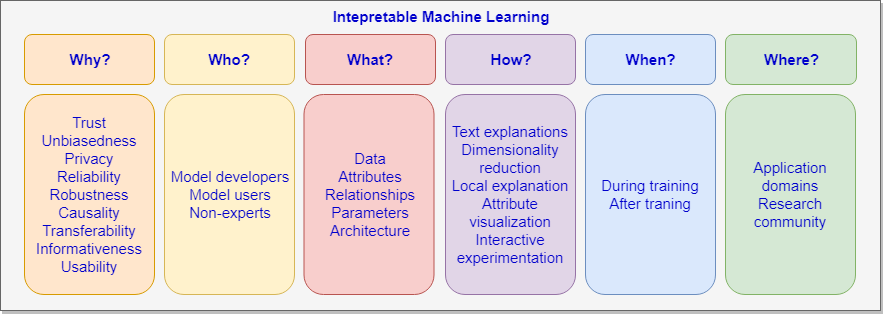
\includegraphics[width=0.9\textwidth]{InterpretableML.png}
 \caption{Aspects to consider when designing Interpretable ML systems.}
 \label{fig:interpretableML}
\end{figure}

Delivering interpretability implies opening the black-box and sometimes it could not be necessary and appropriate to do it, principally when there are no significant consequences for unacceptable results or the problem is sufficiently well-studied and validated in real applications that user trust the system’s decision, even if this is not perfect \cite{Doshi-Velez2017c}.

\subsection{Frameworks for Interpretability}

Some relatively basic techniques for interpret ML models are \cite{Becker2018MachineExplainability}: Permutation importance, for determining which attribute produces the highest performance decrease, and Partial dependence plots, for visualizing influence direction and shape when varying an attribute value.

A more sophisticated technique is LIME \cite{Ribeiro2016}, Local Interpretable Model-Agnostic Explanations, where a specific prediction is explained by learning an interpretable model locally. The result of LIME is a probability for each attribute value of belonging to the prediction class. In addition, the authors show the potential of the framework in applications based on tabular, image and text data. LIME is extended by SHAP \cite{Lundberg2017APredictions}, including an additional component based on the identification of a new class of additive attribute importance measures. LIME is also extended in \cite{Teso2018} and \cite{Phillips2018InterpretableLearning} to explain the query produced in an AL scenario. Local explanations are the base of works focused on produce global interpretation as proposed in \cite{Yang2018}. From contribution matrix representing the attribute importance for every data item, a binary tree is learned to explicitly represent the most important decision rules that are implicitly contained in the black-box model. 

Black-box Deep Learning models have the disadvantage of being the least interpretable because their large number of parameters as measure of complexity. Contributions in this field have been achieved by producing interpretation of the features learned at each layer of a Neural Network \cite{Yosinski2015a},\cite{Olah2018}. A more extensive literature review about interpretability in Deep Learning can be found in \cite{Zhang2018}.

\section{The link between both worlds}
\label{section2.3}

Interactive ML and Interpretable ML in the most of cases previously described has been tackled as isolated concepts. In some scenarios, mechanisms for \textbf{sample review} and \textbf{feedback assignment} (e.g. labeling or parameter tuning) may not be enough to successfully fulfill the user task. \textbf{Model inspection} implies opening the black-box and presenting it to user in an interpretable way and model interpretation indicates the ability to provide explanations about their inner working which could help users to better understand their results \cite{Doshi-Velez2017c}. This extension could support the \textbf{task overview} interface element because, as stated in \cite{Doshi-Velez2017c}, \cite{Lipton2017}, model interpretation is used to achieve other important requirements in user-centric ML systems such as trust, unbiasedness, privacy, reliability, robustness, causality, transferability, informativeness and usability.

In other words, \textbf{an Interactive ML system is not necessarily interpretable in terms of what model is learning and, in the opposite case, an Interpretable ML system could not involve all enough elements of interaction to perform the task in an usable and efficient way}. Designers must not forget the system is constrained by an user task and users are the ones who have the power to determine if the task was effectively fulfilled. User evaluation for interactivity and interpretability, as in any HCI study, must be considered.
